\subsubsection{Communication Port}

The communication port is the only component needed to define a communication layer of the service.
It encapsulates detail needed to express a service, which are the listening protocol, location, and the interfaces. The location of port defines the communication channel for the port. For protocol part, Jolie supports a variety of communication protocols, not only limited to the web protocol like SOAP, HTTP and, SODEP (a Jolie specific binary protocol), it also supports the Bluetooth protocol and in-memory communication. Lastly, the interfaces define a list of operations related to the port depending on type of the port.

A Communication port in Jolie can be classified into two types, whether it is exposing a communication channel to the external service so called an \textit{inputPort}, or it is expressing the communication channel to other service, or the \textit{outputPort}.

Jolie also equipped with the primitives to define the advanced composition of the input port. One of the primitive that is offered by Jolie is \textit{aggregation}, which composes operations from a output port to defining input port and allows an input port to accept operations exposed in the output port. this allows developers to intercept a message between the two ports.

\begin{figure}[ht]
    \begin{framed}
        \begin{grammar}

            <outputPort> ::= `outputPort' \\ <portName> `{' <portConfigurationPair>+ `}'

            <inputPort>
            ::= `inputPort' <portName> `{' ( <portConfigurationPair> | <inputPortConfigurationPair> )+ `}'

            <portConfigurationPair>
            ::= `location' `:' \textit{StringLiteral}
            \alt `protocol' `:' <ID>
            \alt `interfaces' `:' <interfaceName>

            <inputPortConfigurationPair>
            ::=  `aggregates' `:' <portName> ( `,' <portName> )* \alt \dots

            <portName> ::= <ID>
            <interfaceName> ::= <ID>

        \end{grammar}
    \end{framed}
    \caption{Jolie Port Definition Syntax}
\end{figure}

\FloatBarrier

As an example of the concept presented in this section, we create a service as depicted in ~\ref{list:example-port-graphic}.
The service \texttt{program} acts as a producer of the operations in \texttt{personInterface}, where the communication channel is defined in \texttt{personInputPort}.
This service also acts as a consumer of \texttt{loggerInterface} defined by an output port \texttt{LoggerOutputPort}.
One key takeaway from this example is the usage of aggregation at line 11 which makes \texttt{personInputPort} accept the additional operations defined in \texttt{personInterface}. Different scenarios alter the behavior when an aggregated operation is invoked, for this specific example, since the operations in \texttt{loggerInterface} are distinct from the ones defined in the interface of the input port, Jolie will automatically forward the message to the origin aggregation output port.

For the interaction between ports through input/output operations, we will look at again in ~\ref{sec:jolie-behavior}.

\begin{figure}[ht]
    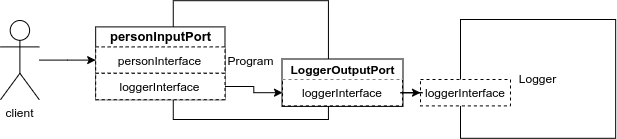
\includegraphics[width=10cm]{ExamplePort}
    \centering
    \caption{A service for port example}
    \label{list:example-port-graphic}
\end{figure}

\begin{listing}[ht]

    \lstset{language=Jolie,
        style=codeStyle,
        numbers=left,
        firstnumber=1
    }
    \begin{lstlisting}[frame=tlrb, caption= {Jolie Port declaration example}, label={list:example-port} ]{port-Jolie}
outputPort LoggerOutputPort {
    location: "socket://logger-service-location:3000"
    protocol: sodep
    interfaces: loggerInterface
}

inputPort personInputPort {
    location: "socket://localhost:3000"
    protocol: http
    interfaces: personInterface
    aggregates: Logger
}

main {
    createPerson(person)(result){
        log@LoggerOutputPort(person)
        result = true
    }
}
\end{lstlisting}
\end{listing}

In this section, we briefly show components for expressing a communication port in Jolie. Port can either be expressed as an incoming or outgoing communication. Both consist of fields that together define details for deploying a service, such as the operations and the message structure it accepts, the location it is using, and the communication protocol. Jolie is also equipped with a set of primitives that allow an advanced composition at the communication level, such as aggregation, which aggregates outgoing and incoming port, allowing the incoming port to accept and forward the message to the destination outgoing port.

\FloatBarrier
